\documentclass[final]{elsarticle}
%\usepackage[pdftex,breaklinks,linktocpage,pagebackref,hyperindex,hyperfigures]
\usepackage{hyperref}
\usepackage[utf8]{inputenc}
\usepackage{amsmath}
\usepackage{amsthm}
\usepackage{amssymb}
\usepackage[tmargin=1in,bmargin=1in,lmargin=1in,rmargin=1in]{geometry}
\usepackage{subfigure}
\usepackage{graphicx}
\usepackage{latexsym}
\usepackage{pdfsync}
% \usepackage[boxed]{algorithm}
\usepackage{algpseudocode}
\usepackage{algorithm}
% \usepackage{algorithmic}
\usepackage{multirow}
\usepackage{rotating}
\usepackage{color}
\usepackage{caption}
\usepackage{url}
\usepackage{tikz}
\usepackage{diagbox}
\usepackage{kpfonts}

\DeclareSymbolFont{extraup}{U}{zavm}{m}{n}
\DeclareMathSymbol{\varheart}{\mathalpha}{extraup}{86}
\DeclareMathSymbol{\vardiamond}{\mathalpha}{extraup}{87}


\hypersetup{
    colorlinks=true,      		% false: boxed links; true: colored links
    linkcolor=blue,       		% color of internal links
    citecolor=blue,       		% color of links to bibliography
    filecolor=black,      		% color of file links
    urlcolor=red,       		% color of external links
    pdffitwindow=true,
    pdfpagelayout=SinglePage
}

% defining some new commands
\newcommand{\etal}{\textit{et al.\ }}
\newcommand{\mbf}[1]{\mathbf{#1}}
\newcommand{\comment}[1]{\textcolor{red}{{#1}}}
\newcommand{\mohammad}[1]{\textcolor{blue}{{Mohammad: #1}}}
\newcommand{\tensor}[1]{\underline{\underline{\boldsymbol{#1}}}}
\newcommand{\be}{\begin{equation}}
\newcommand{\ee}{\end{equation}}
\newcommand{\ben}{\begin{equation*}}
\newcommand{\een}{\end{equation*}}
\newcommand{\bea}{\begin{eqnarray}}
\newcommand{\eea}{\end{eqnarray}}
\newcommand{\bean}{\begin{eqnarray*}}
\newcommand{\eean}{\end{eqnarray*}}
\newcommand{\pd}[2]{\frac{\partial #1}{\partial #2}}
\newcommand{\pdn}[3]{\frac{\partial^#1 #2}{\partial #3^#1}}
\newcommand{\noi}{\noindent}
\newcommand{\ind}{\indent}
\newcommand{\divg}[1]{\nabla \cdot \left(#1\right)}
\newcommand{\ddivg}[1]{\nabla \cdot #1}
\newcommand{\non}{\nonumber}
\newcommand{\fcite}[1]{(\textcolor{blue}{cite: #1})}
% \newcommand{\drawcircle}[2]{\protect  \tikz \protect \node[circle,draw,scale=#1,fill=#2] {};}
% \newcommand{\drawsquare}[2]{\protect  \tikz \protect \node[rectangle,draw,scale=#1,fill=#2] {};}
% \newcommand{\drawdiamond}[2]{\protect \tikz \protect \node[rectangle,draw,scale=#1,fill=#2,rotate=45] {};}
\newcommand{\drawcircle}[1]{\textcolor{#1}{$\bullet$}}
\newcommand{\drawsquare}[1]{\textcolor{#1}{$\blacksquare$}}
\newcommand{\drawdiamond}[1]{\textcolor{#1}{$\vardiamond$}}
\newtheorem{property}{Property}

\begin{document}

\title{Parallel Level-set Methods on Adaptive Tree-Based Grids}

\cortext[cor]{Corresponding author: m.mirzadeh@engineering.ucsb.edu}
\address[MECHE]{Department of Mechanical Engineering, University of California, Santa Barbara, CA 93106-5070, United States.}
\address[CS]{Department of Computer Science, University of California, Santa Barbara, CA 93106-5110, United States.}
\address[UBONN]{Institute for Numerical Simulation, University of Bonn, Bonn 53115, Germany.}

\author[MECHE]{Mohammad Mirzadeh\corref{cor}} \author[MECHE]{Arthur Guittet} \author[UBONN] {Carsten Burstedde} \author[MECHE,CS]{Frederic Gibou}

%!TEX root = draft.tex
\begin{abstract}
We present scalable parallel algorithms for the level-set method on adaptive Quadtree and Octree Cartesian grids. The algorithms are based on a domain decomposition technique and implemented using \texttt{MPI} and the open-source \texttt{p4est} library. An important contribution is a scalable parallel semi-Lagrangian method which, similar to its serial implementation, is free of any time-step restrictions. This is achieved by introducing a scalable global interpolation scheme on adaptive tree-based grids. Moreover, we present a simple parallel reinitialization scheme using the pseudo-time transient formulation. Both parallel algorithms scale on the Stampede supercomputer, where we are limited to 4096 cores currently. Finally a relevant application of the algorithms is presented in modeling the crystallization phenomena by solving a Stefan problem, illustrating a level of detail that would be impossible to achieve without a parallel adaptive strategy. We believe that the algorithms presented in this article will be of interest and useful to researchers working with the level-set framework and modeling multi-scale physics in general.
\end{abstract}
\begin{keyword}
Quadtree/Octree Grids \sep Parallel Computing \sep Space Filling Curves \sep Semi-Lagrangian Method \sep Level-set Method
\end{keyword}
\maketitle

%!TEX root = draft.tex
\section{Introduction}\label{sec:introduction}
The level-set method, originally proposed by Sethian and Osher \cite{Osher;Sethian:88:Fronts-Propagating-w}, is a popular and powerful framework for tracking arbitrary interfaces that undergo complicated topological changes. As a result, the level-set method has been used to a wide range of applications such as multiphase flows, image segmentation, and computer graphics \cite{Osher;Fedkiw:02:Level-Set-Methods-an,Sethian:99:Level-set-methods-an}. An important feature of this method is that the location of the interface is defined implicitly on an underlying grid. This convenience, however, comes at a price. First, compared to an explicit method, e.g.\ front tracking \cite{Juric:96:A-Front-Tracking-Met, Tryggvason;Bunner;Esmaeeli;etal:01:A-Front-Tracking-Met}, the level-set method is typically less accurate and mass conservation could be a problem, although progress has been made in resolving this issue \cite{Enright;Fedkiw;Ferziger;etal:02:A-Hybrid-Particle-Le}. Second, the level-set function has to be defined in a one dimension higher space than that of the interface. If only the location of the interface is needed, the added dimension greatly increases the overall computational cost for uniform grids. One way to avoid this problem is by computing the level-set only close to the interface, e.g.\ as in the narrow-band level-set method \cite{Adalsteinsson;Sethian:95:A-Fast-Level-Set-Met} or, more recently, by using a hash table to restrict both computation and storage requirements \cite{Brun;Guittet;Gibou:12:A-local-level-set-me}.

Another approach that can address both problems is the use of local grid refinement. In \cite{Strain:99:Tree-Methods-for-Mov} the idea of using tree-based grids for level-set calculations was first introduced and later extended in \cite{Popinet:03:Gerris:-A-Tree-Based, Losasso;Gibou;Fedkiw:04:Simulating-Water-and} for fluid simulations. More recently, authors in \cite{Min;Gibou:07:A-second-order-accur} proposed second-order accurate level-set methods on Quadtree (two spatial dimensions) and Octree (three spatial dimensions) grids. The use of adaptive tree-base grids in the context of the level-set method is quite advantageous because (i) it gives fine-grain control over errors, which typically occur close to the interface and (ii) it can effectively reduce the dimensionality of the problem by focusing most of the grid cells close to the interface. Fortunately, constructing the tree is quite simple in the presence of an interface that naturally defines an ideal metric for refinement. However, even though the use of adaptive grids can dramatically reduce the computational cost, performing high-resolution three dimensional calculations of complex interfacial problems, e.g.\ crystal growth in binary alloys \cite{Theillard;Gibou;Pollock:14:A-Sharp-Computationa}, could be prohibitively expensive or even impossible on a serial machine.
In this paper we extend the level-set technology on Quad-/Octrees by proposing
parallel algorithms for distributed memory machines using a domain
decomposition technique.

One of the main challenges in parallelizing algorithms on adaptive grids is
handling the grid itself.
One option is to replicate the entire grid on each process and to employ serial
ordering techniques, as originally implemented by the \texttt{deal.II} library
\cite{Bangerth;Hartmann;Kanschat:07:deal.II----a-General}, or serial
graph partitioners such as METIS \cite{KarypisKumar95}.
%
% off-the-shelf graph partitioners, e.g.\ ParMetis
% \cite{Karypis;Kumar:98:A-parallel-algorithm} or Zoltan
% \cite{Boman;Catalyurek;Chevalier;etal:12:The-Zoltan-and-Isorr}, for load
% balancing and domain decomposition.
% For instance, this was the approach originally taken by the \texttt{deal.II}
% library \cite{Bangerth;Hartmann;Kanschat:07:deal.II----a-General}.
%
This approach, however, is only scalable to a few hundred processes at best and
is limited by the size of the grid itself that can fit in memory.
Even though parallel general-purpose partitioners have since been popularized
\cite{Karypis;Kumar:98:A-parallel-algorithm,
Boman;Catalyurek;Chevalier;etal:12:The-Zoltan-and-Isorr} and
the scalability of partitioning algorithms for unstructured grids
has been improved (see e.g.\ \cite{SahniZhouShephardEtAl09}),
% the use of a general-purpose graph partitioner
their use
adds extra overhead that can limit the overall scalability.
Interestingly, tree-based grids have a nice spatial ordering that naturally
leads to the concept of space-filling curves (SFCs) and can be efficiently
exploited for parallel load balancing
\cite{Aluru;Sevilgen:97:Parallel-domain-deco, GriebelZumbusch99,
      Campbell;Devine;Flaherty;etal:03:Dynamic-octree-load-}.

The idea of using SFCs for parallel partitioning of Quad-/Octrees is not new in itself and has been used by many researchers. For instance, \texttt{Octor} \cite{Tu;OHallaron;Ghattas:05:Scalable-parallel-oc} uses a Morton curve (also known as Z-curve) for traversing the leaves of an Octree for indexing and load balancing and has been scaled up to 62,000 cores \cite{Burstedde;Ghattas;Gurnis;etal:08:Scalable-adaptive-ma}.
\texttt{Dendro} \cite{Sampath;Adavani;Sundar;etal:08:Dendro:-parallel-alg} is
an example of a so-called linear Octree code in which new algorithms are
introduced for parallel partitioning and the development of a parallel
geometric multigrid that has been scaled up to about 32,000 cores
\cite{Sampath;Biros:10:A-parallel-geometric}.
More recently, authors in
\cite{Burstedde;Wilcox;Ghattas:11:p4est:-Scalable-Algo} extended these ideas by
optionally allowing for a collection, or a ``forest'', of connected Octrees,
% that are connected through a common, potentially unstructured, hexahedral grid.
which is partitioned in parallel using a global Morton curve.
%
% \textcolor{red}{How about adding the p4est comments here ?}
%
% An implementation of these algorithms is publicly available
%
% provides a simple API for handling the grid.
The \texttt{p4est} library \cite{p4est-github} provides a publicly available
implementation of these algorithms that is equally efficient for a single tree
as well as multiple trees and has been shown to scale to more than
% 200,000 cores,
450,000 CPU cores \cite{IsaacBursteddeWilcoxEtAl15}.
In fact, the algorithms presented in this paper are implemented on top of
the \texttt{p4est} API.
Due to the need for multiple adaptation and partitioning operations in each
time step, the semi-Lagrangian method we describe below presents a stringent
test of the algorithms and implementation both in terms of scalability and
absolute run time.
% using a single octree to represent the unit cube.
% In fact, the algorithms presented in this paper are implemented on top of the
% \texttt{p4est} library \cite{p4est-github} that is publicly available and
% provides a simple API for handling the grid.
%
% and we do not discuss any algorithm that is already covered in
% \cite{Burstedde;Wilcox;Ghattas:11:p4est:-Scalable-Algo}.

Parallel level-set algorithms can be categorized into two groups: parallel advection algorithms and parallel reinitialization algorithms. Eulerian advection schemes can easily be parallelized but unfortunately are limited by the CFL condition, which could be very restrictive for adaptive grids. Semi-Lagrangian methods combine the unconditional stability of Lagrangian methods and the ease of use of Eulerian grids and have been successfully used for advecting the level-set function on tree-based grids \cite{Losasso;Gibou;Fedkiw:04:Simulating-Water-and, Losasso;Fedkiw;Osher:06:Spatially-Adaptive-T, Min;Gibou:07:A-second-order-accur}. However, parallelizing the semi-Lagrangian algorithm in a domain decomposition context is not an easy task.
The reason for this is twofold.
First, depending on the CFL number, the departure points may end up outside the
ghost region and in remote processes that are potentially far away.
This requires a very dynamic and nonuniform communication pattern that is
challenging to implement.
For an adaptive grid, the situation is even more complex due to the asymmetric
nature of the communication pattern (cf.\ section \ref{sec:parallel
algorithms}).
Second, load balancing could be an issue for large CFL numbers and nonuniform
velocity fields, due to clustering of departure points, which can thus
considerably restrict the scalability of the algorithm. Both of these problems,
of course, could be avoided by choosing $\text{CFL} \le 1$ but that would
defeat the purpose of using the semi-Lagrangian algorithm in the first place.

Nonetheless, several parallel semi-Lagrangian algorithms have been proposed.
A simple domain decomposition technique was used in
\cite{Thomas;Cote:95:Massively-parallel-s} where the width of the ghost layer
is fixed based on the maximum CFL number to ensure that all departure points
are covered by the ghost layer.
Good scalings were reported for small CFL numbers ($\text{CFL} \le 2$).
However, for large CFL numbers, this leads to a large volume of communication that can limit the scalability. In \cite{Drake;Foster;Michalakes;etal:95:Design-and-performan} the authors propose a more sophisticated domain decomposition approach which uses a ``dynamic ghost layer''. Here the width of the ghost layer is dynamically determined at runtime based on information from previous time steps. Unfortunately, this approach also suffers from excessive communication overhead at large numbers of processes. More recently, the authors in \cite{White-III;Dongarra:11:High-performance-hig} used a domain decomposition strategy on a cubed sphere but with a single layer of ghost nodes. Interpolation on remote processes is then handled by sending query points to the corresponding process and asking for the interpolated result. This approach seems to provide good scalability for transporting a single tracer up to about 1000 cores for $\text{CFL} \sim 10$. At higher CFL numbers, the method begins to loose scalability due to an increase in communication volume. Finally, note that although we are mainly interested in parallel semi-Lagrangian methods, one could resort to finite difference or finite element discretization methods if small CFL numbers are acceptable. Indeed several algorithms of this type have been proposed with applications to modeling dendritic crystal growth \cite{Wang;Chang;Kale;etal:06:Parallelization-of-a}, multiphase flows \cite{Sussman:05:A-parallelized-adapt, Fortmeier;Bucker:11:A-parallel-strategy-, Rodriguez;Sahni;Lahey-Jr;etal:13:A-parallel-adaptive-}, and atomization process \cite{Herrmann:10:A-parallel-Eulerian-}.
%, and image segmentation on GPUs \cite{Lefohn;Cates;Whitaker:03:Interactive-GPU-base,Cates;Lefohn;Whitaker:04:GIST:-an-interactive,Roberts;Packer;Sousa;etal:10:A-work-efficient-GPU}.

In many applications, it is desirable that the level-set function has the signed-distance property, i.e., $|\nabla \phi| = 1$. Generally, there are two approaches to enforce this property, either by solving the pseudo-time transient reinitialization equation \cite{Sussman;Smereka;Osher:94:A-Level-Set-Approach, Osher;Fedkiw:01:Level-Set-Methods:-A}
\ben
\phi_\tau + S(\phi_0)\left(|\nabla \phi| - 1\right) = 0,
\een
or by solving the Eikonal equation
\ben
F(x)|\nabla\phi| = 1
\een 
with constant speed function $F(x) \equiv 1$. The transient reinitialization equation can be solved using explicit finite differences and thus can easily be parallelized in a domain decomposition approach. Moreover, only a few iterations may be needed if the signed-distance property is only required close to the interface \cite{Min;Gibou:07:A-second-order-accur}. This is the approach we have chosen in this paper. However, if the signed-distance property is required in the entire domain, solving the Eikonal equation is more computationally efficient. Unfortunately, the most popular algorithm for solving the Eikonal equation, i.e.\ the Fast Marching Method \cite{Sethian:96:A-Fast-Marching-Leve,Sethian:99:Level-set-methods-an}, is inherently sequential due to causal relationship between grid points and cannot be easily parallelized.
The Fast Sweeping Method (FSM) \cite{Zhao:05:A-fast-sweeping-meth} is an
alternative for solving the Eikonal equation iteratively.
The FSM can be more computationally efficient for simple choices of speed
function, e.g.\ as in this context, and for simple interfaces.
Moreover, FSM has more potential for parallelization compared to the FMM.

One of the earliest attempt in parallelizing the FMM is reported in \cite{Herrmann:03:A-domain-decompositi} where a domain decomposition algorithm was introduced. Unlike the serial FMM, however, parallel FMM potentially requires multiple iterations or ``rollback operations'' to enforce causality across processes. Similar ideas are described in detail in \cite{Tugurlan:08:Fast-marching-method}. It should be noted that the number of iterations needed for the parallel FMM to converge greatly depends on the complexity of the interface and on the parallel partitioning and, in general, fewer iterations are required if the domains are aligned with the normals to the interface. Due to the nature of the Eikonal equation, shared memory machines might be a better environment for parallelization. For instance, in \cite{Breus;Cristiani;Gwosdek;etal:11:An-adaptive-domain-d} the authors use an ``adaptive'' technique where individual threads implicitly define a domain decomposition at runtime. Unfortunately, this approach does not seem to be more effective than a simple static decomposition. In \cite{Zhao:07:Parallel-implementat} a parallel FSM method was presented for the first time, which suffered from a plateau in the speedup. A scalable FSM was more recently proposed in \cite{Detrixhe;Gibou;Min:13:A-parallel-fast-swee}, where the Cuthill-McKee numbering was utilized to improve scalability.  A two-scale, hybrid FMM-FSM was presented in \cite{Chacon;Vladimirsky:13:A-parallel-Heap-Cell} which, albeit being more complicated to implement, promises even better scalability. Finally, a parallel Fast Iterative Method (FIM) was proposed in \cite{Jeong;Whitaker:08:A-fast-iterative-met}. The FIM is similar to FMM in that it also maintains a list of ``active nodes''. However, unlike FMM, FIM avoids sorting the list and allows for concurrent updating of all nodes in an iterative fashion. In this article we choose the pseudo-time transient formulation for two reasons: 1) it is considerably easier to parallelize on Quadtrees and Octrees and 2) we are merely interested in the signed-distance property close to the interface, which only requires a few iterations.

This article is organized as follows: In section \ref{sec:levelset method}, we briefly review the sequential algorithms and discretization methods for the level-set equation on adaptive tree-based grids. These ideas are then extended in section \ref{sec:parallel algorithms} to parallel environments using a domain decomposition method. In section \ref{sec:scaling}, we provide several examples that illustrate the scalability of our algorithms. Finally, we close by providing an application of our method by considering the simulation of the solidification process by solving a Stefan problem in section \ref{sec:application}.

%!TEX root = draft.tex
\section{The level-set method}\label{sec:levelset method}
The level-set method, introduced in \cite{Osher;Sethian:88:Fronts-Propagating-w}, is an implicit framework for tracking interfaces that undergo complicated topological changes. In this framework an interface is represented by the zero contour of a higher dimensional function, e.g. a curve in two spatial dimension can be described as $\Gamma = \{(x,y) | \phi(x,y) = 0\}$ where $\phi(x,y)$ is the level-set function. The evolution of the curve under a velocity field $\mathbf{V}$ is then obtained by solving the level-set equation:
\be
\phi_t + \mathbf{V} \cdot \nabla \phi = 0.
\label{eq:ls}
\ee
When the velocity field does not depend on the level-set function itself, equation \eqref{eq:ls} can be solved using the Semi-Lagrangian method. An important advantage of the Semi-Lagrangian method over the regular finite difference method is its unconditional stability which allows for arbitrarily large time steps. This is particularly important when using adaptive grids that allow for higher grid resolutions.

In general, an infinite number of level-set functions can describe the same zero contour and thus interface. However, it is desirable to chose a function with the signed distance property, i.e. $|\nabla \phi| = 1$. As detailed in section \ref{sec:introduction}, we solve the pseudo-time transient reinitialization equation \cite{Sussman;Smereka;Osher:94:A-Level-Set-Approach, Osher;Fedkiw:01:Level-Set-Methods:-A} to achieve this property,
\be
\phi_\tau + S(\phi_0)\left(|\nabla \phi| - 1\right) = 0,
\label{eq:reinitialization}
\ee
where $\phi_0$ is any level-set function that correctly describes the interface location and $S(\phi_0)$ is an appropriate approximation of the sign function \cite{Osher;Fedkiw:02:Level-Set-Methods-an}. Here, we do not go into the details of the sequential algorithms for solving equations \eqref{eq:ls} and \eqref{eq:reinitialization}. Instead, we note that the algorithms presented in section \ref{sec:parallel algorithms} are based on the sequential methods presented in \cite{Min;Gibou:07:A-second-order-accur} and refer the interested reader to the aforementioned article and references therein for more details.

% \indent The level-set method is a method to capture interfaces implicitely by constructing a function $\phi$, called the level-set function, that is negative on on side of the domain $\Omega^-$ and positive on the other side $\Omega^+$, thus defining the interface $\Gamma$ as the zero contour of $\phi$, $\Gamma = \{\mathbf{x} \vert \phi(\mathbf{x}=0\}$.\\

% If infinitely many functions satisfy these requirements, the most natural and most convenient representation is a signed distance function to the interface. The level-set function is therefore reinitialized to a signed distance function at every time step by solving the reinitialization equation

% \begin{equation} \label{eq::reinitialization}
% \pd{\phi}{\tau} + \mathrm{sign}(\phi) \left( \lvert \phi \rvert - 1 \right) = 0,
% \end{equation}

% where $\tau$ is a fictitious time. The discretization and implementation of this procedure will be discussed later in section \ref{section::reinitialization}. Geometrical quantities such as the normal to the interface and the local curvature can be computed straightforwardly from the level-set function as

% \begin{equation*}
% \mathbf{n} = \frac{\nabla \phi}{\lvert \nabla \phi \rvert},
% \end{equation*}

% where it should be noted that $\lvert \nabla \phi \rvert = 1$ when the level-set function is reinitialized, and

% \begin{equation*}
% \kappa = \nabla \cdot \mathbf{n} =  \nabla \cdot \left( \frac{\nabla \phi}{\lvert \nabla \phi \rvert} \right).
% \end{equation*}


% \section{The \texttt{p4est} library}

% The work we present relies on the parallel octree library \texttt{p4est} \cite{Burstedde;Wilcox;Ghattas:11:p4est:-Scalable-Algo}. It is scalable implementation of the general octree structure in a massively parallel mpi environment. We limit our presentation of \texttt{p4est} to the relevant information for our application, for more details the reader is invited to read the original article \cite{Burstedde;Wilcox;Ghattas:11:p4est:-Scalable-Algo}.

% The \texttt{p4est} library provides the geometrical information for the leaves of an octree which includes the neighboring information for the leaves (called quadrants in the original article) of the tree, a layer of ghost quadrants and ghost vertices for each process, the coarsening and refining procedures, and encapsulates the communication between processes. However, it does not provide the vertical structure of the octrees. If it is generally unnecessary, it is a desirable feature for a finite differences based code as it speeds up the access to arbitrary quadrants information dramatically. Thus, we choose to reconstruct the local vertical structure of the octree on every processes. Note that given the local and ghost layer information, this is an entirely local procedure and no communication is needed.

% In addition to the owned and ghost categories, we choose to group the vertices in \textit{local} and \textit{layer} sets. We define the layer vertices as the vertices that are part of another process's ghost layer and the local vertices as the vertices that are not part of any other process's ghost layer. Figure \ref{fig::local_layer_vertices} gives a graphical representation of a boundary between two processes and the classification of the various quadrants and vertices. The idea behind this sorting is that layer vertices are needed by other processes for finite difference calculations and therefore require to be synchronized while the local vertices are used only by the process they belong to. We make use of this classification to implement scalable algorithms for the level-set method, as explained in the following sections.

% \begin{figure}[ht!]
% \begin{center}
% \includegraphics[width=.4\textwidth]{pictures/layer_nodes.pdf}
% \caption{Illustration of a possible layout at the interface between two processes. The red quarants and the orange and purples vertices belong to process 1 while the green quadrants and the green and black vertices belong to process 2. The green G denotes the ghost quadrants for process 2, the green dots are the ghost vertices for process 1, and the purple dots correspond to layer vertices for process 1 (and therefore ghost vertices for process 2).} \label{fig::local_layer_vertices}
% \end{center}
% \end{figure}
%!TEX root = draft.tex
\section{Parallel algorithms}\label{sec:parallel algorithms}

To achieve a good parallel performance of our numerical solver, we must ensure
the sufficient scalability of all components.  This observation prompted the
dedicated development and optimization of several techniques, which we discuss
in the present section.

\subsection{Grid management}

Adaptive tree-based grids can significantly reduce the computational cost of
level-set methods by restricting the fine grid close to the interface where it
is most needed \cite{Strain:99:Tree-Methods-for-Mov}.
Moreover, adaptive tree-based grids are easy to generate in the presence of a
signed-distance level-set function \cite{Min;Gibou:07:A-second-order-accur} and
can efficiently be encoded using a tree data structure
\cite{Samet:90:Applications-of-Spat}.
In order to develop scalable parallel algorithms on these grids, it is
necessary to parallelize the data structure and grid manipulation methods such
as refinement and coarsening of cells as well as to provide a fast method for
grid partitioning and load balancing.
The \texttt{p4est} library \cite{p4est-github} is a collection of such parallel
algorithms that has recently emerged and shown to scale up to 458,752 cores
%\cite{Burstedde;Wilcox;Ghattas:11:p4est:-Scalable-Algo}.
\cite{IsaacBursteddeWilcoxEtAl15}.

In \texttt{p4est} the adaptive grid is represented as a non-overlapping collection of trees that are rooted in individual cells of a common coarse grid (cf.\ Figure \ref{fig:p4est_zcurve}). This common coarse grid, which we will refer to as the ``macromesh'', can in general be an unstructured quadrilateral mesh, in two spatial dimensions, or hexahedral mesh, in three spatial dimensions.
In this article, however, it is sufficient to limit discussions to simple
uniform Cartesian macromeshes.
Moreover, it is implicitly assumed that the macromesh is small enough that it
can be entirely replicated on all processes.
For instance, in many of the applications that we are considering in this paper the macromesh is simply a single cell.
\texttt{p4est} allows for arbitrary refinement and coarsening criteria through defining callback functions.
In this article the refinement criteria is chosen based on the distance of individual cells to the interface.
Specifically, a cell $C$ is marked for refinement if
\be
\min_{v \in V(C)} |\phi (v)| \le \frac{L D}{2},
\label{eq:refine}
\ee
where $V(C)$ denotes the set of all vertices of cell $C$, $L$ denotes the
Lipschitz constant of the level-set function, and $D$ denotes the diagonal size
of cell $C$.
Conversely, an existing cell is marked for coarsening if
\be
\min_{v \in V(C)} |\phi (v)| > L D.
\label{eq:coarsen}
\ee
We refer to section 3.2 of
\cite{Burstedde;Wilcox;Ghattas:11:p4est:-Scalable-Algo} for details on the
parallel refinement and coarsening algorithms implemented in \texttt{p4est}.

Once the grid is adapted to the interface, it must be partitioned to ensure
load balancing across processes.
This is achieved by constructing a Z-curve that traverses the leaves of all
trees in order of the tree index (cf.\ Figure \ref{fig:p4est_zcurve}).
A Z-curve is a Space Filling Curve (SFC) with the important property that cells
with close Z-indices are also geometrically close (on average) in the physical
domain.
This is beneficial since it leads to both a reduction in MPI communications and
improvements of the cache performance of several algorithms such as
interpolation and finite difference calculations.
For more details on parallel partitioning in \texttt{p4est} one may refer to
section 3.3 of \cite{Burstedde;Wilcox;Ghattas:11:p4est:-Scalable-Algo}.
\begin{figure}[hbtp]
\begin{center}
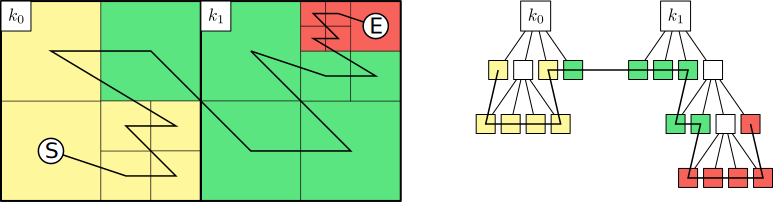
\includegraphics[width = \columnwidth]{figures/p4est_zcurve.pdf}
\caption{Left: a ``forest'' made up of two trees $T_0$ and $T_1$. Parallel
partitioning is achieved by first constructing a Z-curve starting at cell ``S''
and ending at cell ``E''.  Next, the one dimensional curve is split up among
processes either uniformly or by assigning different weights to cells.  Here
processes are represented via different colors.  Note how using the Z-curve
naturally leads to clustering of most cells in each domain.  Right: schematic of
a tree data structure representing this forest and its partitioning.}
\label{fig:p4est_zcurve}
\end{center}
\end{figure}
Aside from grid manipulation and partitioning, we use two additional features
of \texttt{p4est}, namely the generation of ghost layer cells and the creation
of a globally unique node indexing.
These algorithms are detailed in sections 3.5 and 3.6 of
\cite{Burstedde;Wilcox;Ghattas:11:p4est:-Scalable-Algo}.
We have specifically extended the latter algorithm such that it can be applied
to a non-graded refinement pattern.
This is important because we can entirely skip the 2:1 balance function, which
was shown to be one of the most time consuming parts of grid adaptation
in \texttt{p4est}
\cite{Burstedde;Wilcox;Ghattas:11:p4est:-Scalable-Algo}.
% (it has since been optimized \cite{IsaacBursteddeGhattas12}).

Finally, in \texttt{p4est} trees are linearized, i.e.\ only the leaves are explicitly stored. However, explicit knowledge of the hierarchal structure of the tree is greatly beneficial in several algorithms, e.g. in search operations needed for the interpolation algorithm. Thus, we introduce a simple reconstruction algorithm that recreates a local representation of the entire ``forest'' that is only adapted to local cells and, potentially, the ghost layer. This approach is similar to the ideas introduced in \cite{Bangerth;Burstedde;Heister;etal:11:Algorithms-and-data-} and our tests show that in a typical application they amount to less that $1\%$ of the entire runtime. Algorithm \ref{alg:reconstruction} illustrates how this reconstruction is performed. Given a forest and a layer of ghost cells from \texttt{p4est}, the algorithm generates a local representation of the forest by recursively refining from the root until reaching the same level and location of all leaves in the local forest and the ghost layer. Note that algorithm \ref{alg:reconstruction} does not involve any communication and is load balanced provided that the initial forest is balanced. Figure \ref{fig:reconstruction} illustrates an example where Algorithm \ref{alg:reconstruction} is applied. Note how each process has independently generated a local representation of the forest that is refined to match the same leaves as in the global forest and ghost layer.
\begin{figure}[htbp]
\begin{center}
\includegraphics[width = \textwidth]{figures/reconstruct.pdf}
\end{center}
\caption{Left: a forest refined close to an interface and partitioned among four processes, as indicated by colors. Right: each process independently recreates a local forest that is refined to match the local grid and is as coarse as possible elsewhere. Note that empty cells are fictitious, i.e.\ they are only required to generate the hierarchal structure and are not matched by any corresponding cell in the global forest.}
\label{fig:reconstruction}
\end{figure}
\begin{algorithm}[htbp]
\caption{$H \gets \texttt{Reconstruct (}G\texttt{)}$: construction of the local tree hierarchy $H$ from the grid $G$}
\begin{algorithmic}[1]
\State $H \gets G.\texttt{macromesh()}$
\For {$\mathit{tr} : G.\texttt{local\_trees()}$} \Comment{build hierarchy for local cells}
	\For {$c : \mathit{tr}.\texttt{cells()}$}
		\State $H.\texttt{update\_tree(} \mathit{tr}, c \texttt{)}$
	\EndFor
\EndFor

\For {$c : G.\texttt{ghost\_cells()}$} \Comment{build hierarchy for ghost cells}
	\State $H.\texttt{update\_tree(} c.\texttt{tree()}, c \texttt{)}$
\EndFor

\State \Return $H$
\\
\Function{$H.\texttt{update\_tree}$}{$\mathit{tr}, c$}   \Comment{recursive tree reconstruction}
	\State $c_l \gets H.\texttt{root(}\mathit{tr}\texttt{)}$
	\While{$c_l.\texttt{level()} \not= c.\texttt{level()} $}
		\If {$c_l.$\texttt{is\_leaf()}} $c_l$\texttt{.split()}
		\EndIf
		\State $h \gets c_l.\texttt{length()} / 2$ \Comment{select the next child based on direction}
		\State $i \gets c.x \ge c_l.x + h$
		\State $j \gets c.y \ge c_l.y + h$
		\State $k \gets c.z \ge c_l.z + h$

		\State $c_l \gets c_l.\texttt{child(} i, j, k \texttt{)}$
	\EndWhile	
\EndFunction
\end{algorithmic}
\label{alg:reconstruction}
\end{algorithm}

\subsection{Interpolation and semi-Lagrangian methods}
As indicated earlier, we use the semi-Lagrangian method to solve equation \eqref{eq:ls} when the velocity field is externally generated, i.e.\ when it does not depend explicitly on the level-set function itself. Let us rewrite equation \eqref{eq:ls} along the characteristic curve $\underline{\mathbf{X}}(t)$ as:
\be
\left\{
\begin{array}{rcl}
\dfrac{\text{d} \underline{\mathbf{X}}}{\text{d} t} &=& \underline{\mbf{u}}, \\ [3ex]
\dfrac{\text{d} \phi(\underline{\mathbf{X}}(t), t)}{\text{d} t} &=& 0.
\end{array}
\right.
\label{eq:sl}
\ee
The semi-Lagrangian method integrates equations \eqref{eq:sl} backward in time,
i.e.\ starting from the grid $G^{n+1}$ (computed in iteratively as explained
later on), we simply write $\phi^{n+1}(\underline{\mathbf{X}}^{n+1}) =
\phi(\underline{\mathbf{X}}(t^{n+1}), t^{n+1}) =
\phi(\underline{\mathbf{X}}(t^n), t^n) = \phi^n(\underline{\mathbf{X}}_d)$.
Here, the characteristic curves are chosen such that $\underline{\mathbf{X}}(t^{n+1})$ are simply the coordinates of grids points of $G^{n+1}$, and $\underline{\mathbf{X}}_d$ are the departure points, which are computed using the second-order midpoint method \cite{Min;Gibou:07:A-second-order-accur}:
\bea
\underline{\mathbf{X}}^\star &=& \underline{\mathbf{X}}^{n+1} - \frac{\Delta t}{2} \underline{\mbf{u}}^{n}(\underline{\mathbf{X}}^n),	   \label{eq:xstar}      \\
\underline{\mathbf{X}}_d     &=& \underline{\mathbf{X}}^{n+1} - \Delta t \underline{\mbf{u}}^{n+\frac{1}{2}}(\underline{\mathbf{X}}^\star), \label{eq:xdeparture}
\eea
where $\underline{\mbf{u}}^{n+\frac{1}{2}}$ is obtained via extrapolation from previous times, i.e.:
\be
\underline{\mbf{u}}^{n+\frac{1}{2}} = \frac{3}{2} \underline{\mbf{u}}^n - \frac{1}{2}\underline{\mbf{u}}^{n-1}. \label{eq:vn_p_half}
\ee
Note that all values at the intermediate point, $\underline{\mathbf{X}}^\star$,
and departure point, $\underline{\mathbf{X}}_d$, must be calculated via
interpolation from the previous grids $G^{n}$ and $G^{n-1}$.
Here, we use the stabilized second-order interpolation for
$\phi(\underline{\mathbf{X}}_d)$ and the multi-linear interpolation for
$\underline{\mbf{u}}^{n+\frac{1}{2}}(\underline{\mathbf{X}}^\star)$
\cite{Min;Gibou:07:A-second-order-accur}.
Although parallelization of the interpolation process on a shared-memory
machine is trivial, the same cannot be said for distributed-memory machines.
In fact, the parallel interpolation given in Algorithm \ref{alg:interpolation}
is probably the most important contribution of this article since this
procedure, which is trivial on uniform grids, is challenging in the case of
trees because it is not straightforward to identify which processes owns the
departure points.
Indeed, complications arise because not all departure points will reside in the
domain owned by the current process. Moreover, due to the irregular shapes of
the partitions, one cannot even ensure they are entirely owned by neighboring
processes.
At best we can only expect that their locations are bounded by a halo of width
$w \le \text{CFL} \: \Delta x_{\min}$ around the local partition, where
$x_{\min}$ is the size of the smallest cell in the forest.
Naturally, if one enforces $\text{CFL} \le 1$, one can ensure that the halo is
bounded by the ghost layer, which significantly simplifies the communication
problem.
This assumption, however, defeats the purpose of using a semi-Lagrangian
approach, whose purpose is to enable large CFL values.

One remedy to this problem, proposed in \cite{Thomas;Cote:95:Massively-parallel-s} for uniform grids, is to increase the size of ghost layer to $\lceil \text{CFL} \rceil$. For large values of the $\text{CFL}$ number, however, this approach can substantially increase the communication volume. Moreover, this simple approach does not work in the process of generating $G^{n+1}$ due to repartitioning. Indeed, $G^{n+1}$ is built iteratively and load balancing is enforced by repartitioning at each sub-iteration. Therefore, after one such sub-iteration, the backtracked points can end up outside of the initial ghost layer. An alternative approach would be to handle local and remote interpolations separately. Our remote interpolation algorithm is composed of three separate phases. In the first phase, which we call buffering, every process searches for all departure points inside the local trees. If the point is owned by a local cell, it is added to a local buffer, otherwise we find the process which owns the point and add the point to a separate buffer belonging to the found rank. Note that searching the point in the local tree is performed recursively using the hierarchal reconstruction (cf.\ algorithm \ref{alg:reconstruction}). Moreover, the owner's rank is found by computing the Z-index of the point and then using a binary search on the Z-curve. This is already implemented in \texttt{p4est} and explained in details in section 2.5 of \cite{Burstedde;Wilcox;Ghattas:11:p4est:-Scalable-Algo}.

Once buffering is done, every process knows exactly how many messages it needs to send and to which processes. This also implicitly defines processes that will later on send a reply message to this process. However, at this point no process knows which processes to expect a message from. We solve this problem using a simple \textit{communication matrix} (see Figure \ref{fig:communication}). Our approach is very similar to the ``Personalized Census ($\mathcal{PCX}$)'' algorithm described in \cite{Hoefler;Siebert;Lumsdaine:10:Scalable-communication}. Another similar approach is the ``Notify'' algorithm introduced in \cite{Isaac;Burstedde;Ghattas:12:Low-cost-parallel-al}. Furthermore, the MPI-3 standard introduces non-blocking collectives and Remote Memory Access (RMA) operations which enable new ways of solving the communication problem. For instance, authors in \cite{Hoefler;Siebert;Lumsdaine:10:Scalable-communication} descried the ``Non-blocking Consensus ($\mathcal{NBX}$)'' and ``Remote Summation ($\mathcal{RSX}$)'' algorithms which make use of such operations and have better theoretical communication complexities. With the exception of $\mathcal{RSX}$ algorithm, which was not tested in this study, all remaining algorithms produced similar timing and scaling. Thus we have decided to describe our algorithm based on the idea of the \textit{communication matrix}.

\begin{figure}[htbp]
\begin{center}
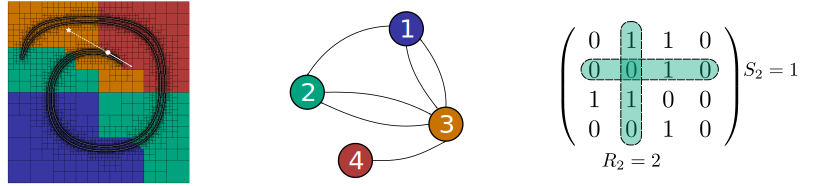
\includegraphics[width = \textwidth] {figures/communication.pdf}
\end{center}
\caption{Left: the location of back-traced points depends on the magnitude of the local velocity and on the time-step. Although the distance to the departure point is bounded by $\text{CFL} \: \Delta x_{\min}$, one cannot predict the receiving rank without explicitly searching the entire Z-curve. Moreover, the receiving process has no prior knowledge about which processes to check for incoming messages nor does it know anything about the possible message length (i.e.\ number of points). Middle: a directed graph illustrating the communication pattern among processes with arrows representing the direction in which messages are sent. Right: the adjacency matrix of the communication graph. For each row, the sum of all columns represents the number of messages that need to be sent. Conversely, for each column, the sum of all rows represents the number of messages that need to be received. As detailed in Algorithm \ref{alg:interpolation}, this information is enough to build a parallel interpolation scheme.}
\label{fig:communication}
\end{figure}

To solve the communication problem, we first compute the adjacency matrix of the communication pattern, i.e.\ we construct the matrix $A_{P \times P}$, where $P$ is the number of processes, such that
\ben
a_{ij} = 
\left\{
\begin{array}{lr}
1 \hspace{5 mm} \text{if process `\textit{i}' sends a message to process `\textit{j}',} \\
0 \hspace{5 mm} \text{otherwise.}
\end{array}
\right.
\een
Note that this matrix is also distributed among processes, i.e.\ each row is owned by a separate rank. Next, we compute
\ben
S_i = \sum_j a_{ij} \hspace{5 mm} \text {and} \hspace{5 mm} R_i = \sum_j a_{ji} ,
\een
where $S_i$ and $R_i$ denote the number of messages sent and received, respectively. While $S_i$ can be computed trivially, a reduction operation is required to compute $R_i$. For instance, this can be achieved using a single \texttt{MPI\_Reduce\_scatter} function call. The last phase of the interpolation procedure involves overlapping the computation of interpolated values for local points with the communication of data between processes. This is done by alternating between local calculations and probing for incoming messages from other processes. The interpolation is finished once the values for all local the points have been calculated and all the remote requests have been processed (see Algorithm \ref{alg:interpolation}).
\begin{algorithm}[htbp]
\caption{$values \gets \texttt{Interpolate (}H, F, \underline{\mathbf{X}}\texttt{)}$: interpolate the value of $F$, defined on the local tree hierarchy $H$, at coordinates $\underline{\mathbf{X}}$}
\begin{algorithmic}[1]
\State $col \gets 0, \mathit{buff} \gets \mathit{null}$ \Comment{Phase I -- buffering}
\For {$\underline{\mathbf{p}} : \underline{\mathbf{X}}$} 
	\State $[r, \mathit{cell})] \gets H.\texttt{search(}\underline{\mathbf{p}}\texttt{)}$ \Comment{search for the owner's rank and cell}
	\If {$r = \mathit{mpirank}$}
        \State $\mathit{buff}[r].\texttt{push\_back(}\underline{\mathbf{p}}, cell\texttt{)}$
	\Else
        \State $\mathit{buff}[r].\texttt{push\_back(}\underline{\mathbf{p}}\texttt{)}$
        \State $\mathit{col}[r] \gets 1$
	\EndIf
\EndFor
\For {$r:\mathit{mpisize}$} \Comment{Phase II -- initiate communication and compute number of messages}
	\If {$\mathit{col}[r]$}
        \State $\texttt{MP\_Isend(}r, \mathit{buff}[r]\texttt{)}$
	\EndIf
\EndFor
\State  $S \gets \texttt{sum(}col\texttt{)}$ 
\State  $R \gets \texttt{MPI\_Reduce\_scatter(}\mathit{col},\texttt{MPI\_SUM)}$
\State $\mathit{done} \gets \mathit{false}, it \gets \mathit{buff}[mpirank].\texttt{begin()}$
\While {$\mathit{!done}$} \Comment{Phase III -- main loop}
	\If {$\mathit{it} \not= \mathit{buff[mpirank]}.\texttt{end()}$}
		\State $\mathit{values} \gets \texttt{process\_local(}it\texttt{)}$ \Comment{process local interpolations}
		\State $\texttt{++}\mathit{it}$
	\EndIf
	\If {$R > 0$} \Comment{process queries sent from remote processes}
		\State $[\mathit{msg, st}] \gets \texttt{MPI\_Iprobe()}$
		\If {$\mathit{msg}$}
			% \State $values \gets \texttt{MPI\_Recv(}st.\texttt{MPI\_SOURCE)}$ \Comment{}
			\State $\mathit{val\_buff} \gets \texttt{process\_queries(}\mathit{st}\texttt{)}$ \Comment{receive, search, and interpolate values}
			\State $\texttt{MPI\_Isend(}\mathit{st}.\texttt{MPI\_SOURCE},\mathit{val\_buff}\texttt{)}$ \Comment{send back interpolated values}
			\State $R\texttt{--}$
		\EndIf
	\EndIf
	\If {$S > 0$} \Comment{process replies sent to our queries}
		\State $\mathit{[msg, st]} \gets \texttt{MPI\_Iprobe()}$
		\If {$\mathit{msg}$}
			\State $\mathit{values} \gets \texttt{process\_replies(}\mathit{st}.\texttt{MPI\_SOURCE)}$ \Comment{receive remotely interpolated values}
			\State $S\texttt{--}$
		\EndIf
	\EndIf
	\State $\mathit{done} \gets S = 0 \: \And \: R = 0 \: \And \: \mathit{it = buff[mpirank]}.\texttt{end()}$
\EndWhile
\State \Return $\mathit{values}$
\end{algorithmic}
\label{alg:interpolation}
\end{algorithm}

Using the interpolation Algorithm \ref{alg:interpolation}, we close this section by presenting the final semi-Lagrangian Algorithm \ref{alg:semi-lagrangian}. The basic idea is to start from an initial guess $G^{n+1}_0$ for the grid and modify it using the refinement \eqref{eq:refine} and coarsening \eqref{eq:coarsen} criteria until convergence is obtained. Various options are available for $G^{n+1}_0$. For instance it is possible to start from the macromesh and only perform refinement steps until convergence. This choice, however, is not suitable since the first few iterations do not contain many cells and there is little work for parallelism. Here we simply take the previous grid as the starting point, i.e.\ $G^{n+1}_0 = G^n$. Note that this iterative process is essentially unavoidable since the grid is based on the values of the level-set function at $t^{n+1}$, which itself is unknown and is to be defined on $G^{n+1}$. Nonetheless the process converges to the final grid in at most $l_{\max}-l_{\min}$ steps where $l_{\min}$ and $l_{\max}$ denote the maximum and minimum depth of all trees in the forest, receptively.
\begin{algorithm}[htbp]
\caption{$[G^{n+1}, \phi^{n+1}] \gets \texttt{SemiLagrangian (}G^n, \phi^n, \underline{\mathbf{u}}^n, \underline{\mathbf{u}}^{n-1}, \text{CFL}\texttt{)}$: update $\phi^{n+1}$ from $\phi^n$ using a semi-Lagrangian scheme and construct the new forest $G^{n+1}$ that is consistent with the zero level-set of $\phi^{n+1}$}
\begin{algorithmic}[1]
\State $\Delta t_l \gets \text{CFL} \times G^n.\texttt{hmin()} / \max \{\underline{\mathbf{u}}^n \} $
\State $\Delta t   \gets \texttt{MPI\_Allreduce(}\Delta t_l,\texttt{MPI\_MIN)}$
\State $H^n \gets \texttt{Reconstruct(} G^n\texttt{)}$ 
\State $G^{n+1}_0 \gets G^n$
\While {$\mathit{true}$}
	\State $\underline{\mathbf{X}}_d  \gets \texttt{ComputeDeparturePoints(}G^{n+1}_0, \underline{\mathbf{u}}^n, \underline{\mathbf{u}}^{n-1}, \Delta t\texttt{)}$ \Comment{using equations \ref{eq:xstar} -- \ref{eq:vn_p_half}}
	\State $\phi^{n+1} \gets \texttt{Interpolate(}H^n, \phi^n, \underline{\textbf{X}}_d\texttt{)}$
	\State $G^{n+1} \gets G^{n+1}_0.\texttt{refine\_and\_coarsen(}\phi^{n+1}\texttt{)}$ \Comment{using equations \ref{eq:refine} and \ref{eq:coarsen} as criteria}
	\If {$G^{n+1} \not= G^{n+1}_0$}
		\State $G^{n+1}.\texttt{partition()}$
		\State $G^{n+1}_0 \gets G^{n+1}$
	\Else
		\State \textbf{break}
	\EndIf
\EndWhile

\State \Return $[G^{n+1}, \phi^{n+1}]$
\end{algorithmic}
\label{alg:semi-lagrangian}
\end{algorithm}

\subsection{Reinitialization}
Successive application of Algorithm \ref{alg:semi-lagrangian}, especially for large values of the CFL number, eventually degrades the signed distance property of the level-set function. Thus, it is important to reinitialize the level-set function every few iterations, especially because the quality of generated grid heavily depends on the signed distance property. To achieve this property we solve the pseudo-time transient equation \eqref{eq:reinitialization} using the discretization scheme detailed in \cite{Min;Gibou:07:A-second-order-accur}. For completeness, we briefly review the scheme. First, we write equation \eqref{eq:reinitialization} in the following semi-discrete form:
\be
\frac{\text{d} \phi}{\text{d} \tau} + S(\phi_0) \left( \mathcal{H}_G(D^+_i \phi, D^-_i \phi) - 1 \right) = 0,
\label{eq:semidiscrete_reinit}
\ee
where $D^+_i \phi$ and $D^-_i \phi$ are the forward and backward derivatives in the $x_i$ direction and $\mathcal{H}_G$ is the Godunov Hamiltonian defined as:
\ben
\mathcal{H}_G(a_i, b_i) = 
\left\{
\begin{array}{lcr}
	\sqrt{\sum_i \max \left(|a^+_i|^2, |b^-_i|^2\right)} & \hspace {5 mm} \text{if} & S(\phi_0) \le 0 ,\\
	\\
	\sqrt{\sum_i \max\left(|a^-_i|^2, |b^+_i|^2\right)} & \hspace {5 mm} \text{if} & S(\phi_0)  >  0 ,
\end{array}
\right.
\een
where $a^+ = \max(a, 0)$ and $a^- = \min(a, 0)$. Similar to \cite{Min;Gibou:07:A-second-order-accur}, equation \eqref{eq:semidiscrete_reinit} is integrated in time using the TVD-RK2 scheme with adaptive time-stepping in order to accelerate the convergence to the steady state. Since the computation is based on a local stencil, the parallel implementation of this scheme is mostly trivial. However, one minor point requires further explanation. As suggested in \cite{Min;Gibou:07:A-second-order-accur}, one-sided derivatives $D^+_i \phi$ and $D^-_i \phi$ are computed using second order discretization which require to compute the second-order derivatives. To enable overlap between computation and communications when computing second-order derivatives and also integrating equation \eqref{eq:semidiscrete_reinit}, we use the following common technique. First, we label all local points, $L_p$, as either private, $P_p$, or boundary, $B_p$. Here, the boundary points are the collection of all local points that are regarded as a ghost point, $G_r$, on at least one other process, i.e.\ $B_p = \underset{r,\;r\neq p}{\bigcup} G_r$. Private points are defined as the collection of all local points that are not a boundary point, i.e.\ $P_p = L_p \setminus B_p$. Algorithm \ref{alg:overlap} illustrates how this labeling can help with overlapping the computation and the communication associated to an arbitrary local operation $y \gets \mathcal{F}(x)$. Note that the \texttt{p4est} library already includes all the primitives required for labeling local points without any further communication.

\begin{algorithm}[htbp]
\caption{$y \gets \texttt{Overlap (}x, \mathcal{F}\texttt{)}$: compute $y_i=\mathcal{F}(x_i)$ for all nodes $i$, where $\mathcal{F}$ is a local operation, while hiding the communication to update the ghost layer}
\begin{algorithmic}[1]
\For {$i:B_p$} \Comment{I -- perform computation on boundary points}
	\State $y_i \gets \mathcal{F}(x_i)$
\EndFor
\State $\mathit{send\_req} \gets \texttt{MPI\_Isend(}y_B\texttt{)}$ \Comment{II -- begin updating ghost values}
\State $\mathit{recv\_req} \gets \texttt{MPI\_Irecv(}y_G\texttt{)}$
\For {$i:P_p$} \Comment{III -- perform computation on private points}
	\State $y_i \gets \mathcal{F}(x_i)$ 
\EndFor
\State $\texttt{MPI\_Waitall(}\mathit{send\_req, recv\_req}\texttt{)}$ \Comment{IV -- wait for ghost update to finish}
\State \Return $y$
\end{algorithmic}
\label{alg:overlap}
\end{algorithm}



\subsection{Accuracy} \label{sec:accuracy}

The numerical methods detailed in the previous sections are widely used in the level-set community and their accuracy is studied for example in \cite{Min;Gibou:07:A-second-order-accur}. However, in order to validate our implementation, we present a brief convergence analysis.

The advection of an irregular boundary using the semi-Lagrangian method is the perfect candidate to demonstrate the accuracy of our implementation as it makes use of the interpolation routine as well as the reinitialization procedure. We select the benchmark problem proposed in \cite{Enright;Fedkiw;Ferziger;etal:02:A-Hybrid-Particle-Le}. Consider a sphere centered at $(0.35,0.35,0.35)$ and with radius $0.15$ in a domain $[0,1]^3$ and deformed under the divergence free velocity field
\be \label{eq:velo_enright}
\begin{cases}
u(x,y,z) = 2 \sin^2(\pi x)\sin(2 \pi y)\sin(2 \pi z), \\
v(x,y,z) = - \sin^2(\pi y)\sin(2 \pi x)\sin(2 \pi z), \\
w(x,y,z) = - \sin^2(\pi z)\sin(2 \pi x)\sin(2 \pi y).
\end{cases}
\ee
forward in time until $t_{1/2}=1$ and then backward to its original state at $t_f=2$. With set the time step to $\Delta t = 5 \Delta x_{min}$, where $\Delta x_{min}$ is the size of the smallest cell in the forest. We monitor the volume loss and the error in the interface location at the final time, when the original shape should be recovered, as the finest resolution of the forest increases. The results are reported in table \ref{tab:accuracy} and figure \ref{fig:accuracy} shows a visualization of the sphere at the initial time, at $t_{1/2}$ when the deformation is maximal, and at the final time. The results are consistent with those reported previously in \cite{Min;Gibou:07:A-second-order-accur} and indicate second order accuracy for the mass loss.

\begin{table}[htbp]
\begin{center}
\begin{tabular}{|c|c|c|c|c|}
\hline
Finest resolution & $L^\infty$ error on $\phi$ & Rate & Volume loss (\%) & Rate \\
\hline
$128^3$  & 1.53E-01 & -    & 1.85E-01 & -    \\
$256^3$  & 1.18E-01 & 0.38 & 3.73E-02 & 2.31 \\
$512^3$  & 9.82E-03 & 3.58 & 6.87E-03 & 2.44 \\
$1024^3$ & 2.56E-03 & 1.94 & 1.92E-03 & 1.84 \\
$2048^3$ & 1.60E-03 & 0.67 & 5.17E-04 & 1.89 \\
\hline
\end{tabular}
\caption{Study of the convergence of the level-set algorithm using Enright's test \cite{Enright;Fedkiw;Ferziger;etal:02:A-Hybrid-Particle-Le}. The $L^\infty$ error on $\phi$ is computed only close to the interface as this is the relevant observable for an advection procedure.} \label{tab:accuracy}
\end{center}
\end{table}

\begin{figure}[htbp]
\begin{center}
\begin{tabular}{ccccc}
\includegraphics[width=.28\textwidth]{figures/enright_0.png}
&
\hspace{.1cm}
&
\includegraphics[width=.28\textwidth]{figures/enright_1.png}
&
\hspace{.1cm}
&
\includegraphics[width=.28\textwidth]{figures/enright_2.png}
\end{tabular}
\caption{Visualization of the deformation undergone by the sphere for the Enright's test at time 0, $t_{1/2}$ and $t_f$ and colored with the processes ranks. The forest's finest resolution is equivalent to a uniform grid with $2048^3$ cells and contains between 17 (at initial and final times) and 63 (at $t_{1/2}$) million nodes. These results were obtained on the Comet supercomputer with 960 processes (40 compute nodes).} \label{fig:accuracy}
\end{center}
\end{figure}
%!TEX root = draft.tex
\section{Scaling} \label{sec:scaling}
In this section we present results that show the scalability of our algorithms. All of our tests have been run on the Stampede cluster at Texas Advanced Computing Center (TACC) where we are limited to $4096$ cores at most. Each node of Stampede has 2 eight-core Xenon E5-2680 processors clocked at 2.7 GHz with 32 GB of DDR3-1600 MHz memory and interconnected using an InfiniBand network card. Unless mentioned otherwise, in all the tests we have used all 16 cores of every node. Finally, in all cases we report the maximum wall time recorded using PETSc's logging interface which has a temporal resolution of roughly $0.1 \: \mu s$.

\subsection{Interpolation}
In this section we show results for a simple test to measure the scalability of the interpolation algorithm \ref{alg:interpolation}. The test consists of interpolating a function at a number of random points on a randomly refined octree in three dimensions. We consider two cases. A small test on a level 9 tree with roughtly 20M cells and 33M nodes and larger test on a level 13 tree with roughly 128M cells and 280M nodes. In both cases number of randomly generated points are chosen to be equal to the number of nodes and the stablized second-order interpolation of \cite{Min;Gibou:07:A-second-order-accur} was performed 10 times to smooth out possible timing fluctuations.

To simulate the effect of different CFL numbers, we generate the random points such that on each processor $\alpha$ percentage of them are located outside the processor boundary and thus will initiate communication. Scaling results are presented for $\alpha = 5 \%$ and $\alpha = 95\%$ for both small and large problems in figure \ref{fig:interpolation}. Excellent scaling is obtained for the small problem for $P = 16-512$ even when $95\%$ of interpolation points are remote to processors. For the larger problem, communication overhead prevents further scaling of algorithm beyond $4096$ processors when $\alpha = 95\%$. Note that for $\alpha = 5\%$, even though some sections of algorithm stop scaling, the overall algorithm still scales since the local work dominates the timing. This illustrates the effectiveness of non-blocking communication pattern in algorithm \ref{alg:interpolation}.

\begin{figure}[htbp]
	\begin{center}
		\subfigure[$N_G = 33$M, $\alpha = 5\%$]{\includegraphics[width = 0.45 \textwidth] {figures/interpolation_small_05.pdf}}
		\subfigure[$N_G = 33$M, $\alpha = 95\%$]{\includegraphics[width = 0.45 \textwidth] {figures/interpolation_small_95.pdf}}
		\\
		\subfigure[$N_G = 280$M, $\alpha = 5\%$]{\includegraphics[width = 0.45 \textwidth] {figures/interpolation_large_05.pdf}}
		\subfigure[$N_G = 280$M, $\alpha = 95\%$]{\includegraphics[width = 0.45 \textwidth] {figures/interpolation_large_95.pdf}}
	\end{center}
	\caption{Strong scaling of algorithm \ref{alg:interpolation} for several tests where $N_G$ denotes the number of random interpolation points (same as number of nodes in the octree) and $\alpha$ denotes the percentage of these points that are remote to each processor. Here ``Total'' represents the total time spent in the interpolation while ``buffer'', ``local'', ``queries'', and ``replies'' represent the the timing for different sections (c.f. algorithm \ref{alg:interpolation}). Results indicate excellent scaling for the small test (a-b) and for the large test when $\alpha = 5\%$ (c). For the extreme case (d) the algorithm stops scaling at $4096$ processors due to communication overhead.}
	\label{fig:interpolation}
\end{figure}

\subsection{Semi-Lagrangian}
To test the scalability of the Semi-Lagrangian algorithm \ref{alg:semi-lagrangian} we consider a slightly modified version of the Enright's rotation test \cite{Enright;Fedkiw;Ferziger;etal:02:A-Hybrid-Particle-Le}, i.e. we advect a sphere of radius 0.35 located at $(0.4, 0.4, 0.4)$ with a divergent free velocity field given by:
\bean
u(x,y,z) &=& 2\sin(\pi x)^2 \sin(2\pi y) \sin(2 \pi z), \\
v(x,y,z) &=& -\sin(\pi y)^2 \sin(2\pi x) \sin(2 \pi z),\\
w(x,y,z) &=& -\sin(\pi z)^2 \sin(2\pi x) \sin(2 \pi y). 
\eean
To understand the effect of CFLnumber on the scalability of the algorithm we perform one step of the Semi-Lagrangian algorithm for $\text{CFL} = 1$, $\text{CFL} = 10$, and $\text{CFL} = 100$. We also perform the test for two set of initial girds, a small grid with $l_\text{max} = 10$ and a larger grid with $l_\text{max} = 12$. After one advection step, each of these grids have approximately 15M and 255M nodes, respectively. 
\begin{table}[htbp]
	\begin{minipage}{.5\linewidth}
		\begin{center}
		\begin{tabular}{|c|cccccc|}
			\hline
				CFL & 16 & 32 & 64 & 128 & 256 & 512 \\
				\hline
				1   & 2 & 2 & 3 & 3 & 3 & 3 \\
				10  & 3 & 3 & 3 & 3 & 3 & 3 \\
				100 & 6 & 6 & 6 & 6 & 6 & 6 \\
			\hline
		\end{tabular}
		\caption*{(a) $l_\text{max} = 10$}
		\end{center}
	\end{minipage}%
	\begin{minipage}{.5\linewidth}
		\begin{center}
		\begin{tabular}{|c|cccccc|}
			\hline
				CFL & 128 & 256 & 512 & 1024 & 2048 & 4096 \\
			\hline
				1   & 3 & 3 & 3 & 3 & 3 & 3 \\
				10  & 3 & 3 & 4 & 4 & 4 & 4 \\
				100 & 6 & 6 & 6 & 6 & 6 & 7 \\
			\hline
		\end{tabular}
		\caption*{(b) $l_\text{max} = 12$}
		\end{center}
	\end{minipage}	
	\caption{Number of iterations required for grid construction in algorithm \ref{alg:semi-lagrangian} for the rotation test on a (a) level-10 and (b) level-12 octree with approximately 15M and 255M nodes, respectively. Note how the iteration count increases with the CFL number but is almost independent of number of processors. The slight dependence of iteration count on number of processors is most likely due to dependence of round-off errors on the number of processors. Nonetheless, close examination of generated octrees (data not shown) reveals that they are identical and independent of the number of processors used to perform the test.}
	\label{tab:semilagrangian}
\end{table}

Table \ref{tab:semilagrangian} illustrates the dependence of number of iterations required to build the grid; as the CFL is increased, interface travels a farther distance which necessitates more iterations to generate the grid. Note that the apparent dependence on the number processors is most likely due to round-off errors during the interpolation and/or backtracking step. Figures \ref{fig:semilagrangian_small} and \ref{fig:semilagrangian_large} illustrate the scalability of the algorithm for small and large problems, respectively. To enable meaningful comparisons between different CFL numbers and number of processors, the maximum time has been scaled to the number of iterations required for grid construction as reported in table \ref{tab:semilagrangian}. For both problems excellent scalability is observed for $\text{CFL} = 1$ and $\text{CFL} = 10$. The algorithm even shows good scalability when taken to the extreme, i.e. for $\text{CFL} = 100$.

An increase in the CFL number has two effects on the algorithm. First, a larger fraction of departure points land in domains of remote processors. Moreover, these points are potentially dispersed across a larger number of processors. This means both the number MPI messages and their volume increases for larger CFL numbers. Second, as more points are shipped to remote processors for interpolation, there is a greater chance that interpolation load is unbalanced across processors. This is specially true for regions of space in which streamlines cluster. Both factors contribute to decrease the scalability of the algorithm at larger CFL numbers. 
\begin{figure}[htbp]
	\begin{center}
		\subfigure[Semi-Lagrangian, $\text{CFL} = 1$]{\includegraphics[width = 0.3 \textwidth] {figures/SL_Small_1_SemiLagrangian.pdf}}
		\subfigure[Semi-Lagrangian, $\text{CFL} = 10$]{\includegraphics[width = 0.3 \textwidth] {figures/SL_Small_10_SemiLagrangian.pdf}}
		\subfigure[Semi-Lagrangian, $\text{CFL} = 100$]{\includegraphics[width = 0.3 \textwidth] {figures/SL_Small_100_SemiLagrangian.pdf}}
		\\
		\subfigure[Interpolation, $\text{CFL} = 1$]{\includegraphics[width = 0.3 \textwidth] {figures/SL_Small_1_Interpolation.pdf}}
		\subfigure[Interpolation, $\text{CFL} = 10$]{\includegraphics[width = 0.3 \textwidth] {figures/SL_Small_10_Interpolation.pdf}}
		\subfigure[Interpolation, $\text{CFL} = 100$]{\includegraphics[width = 0.3 \textwidth] {figures/SL_Small_100_Interpolation.pdf}}
	\end{center}
	\caption{Strong scaling of a single iteration of algorithm \ref{alg:semi-lagrangian} for the rotation test on a level-10 octree with approximately 13M cells and 15M nodes. Top row: scaling of various components of the algorithm for (a) $\text{CFL} = 1$, (b) $\text{CFL} = 10$, and (c) $\text{CFL} = 100$. Bottom row: breakdown of various components of the interpolation phase for the same CFL numbers. Note that the maximum time has been scaled with the number of iterations required to build the tree (c.f. table \ref{tab:semilagrangian}).}
	\label{fig:semilagrangian_small}
\end{figure}

\begin{figure}[htbp]
	\begin{center}
		\subfigure[Semi-Lagrangian, $\text{CFL} = 1$]{\includegraphics[width = 0.3 \textwidth] {figures/SL_Large_1_SemiLagrangian.pdf}}
		\subfigure[Semi-Lagrangian, $\text{CFL} = 10$]{\includegraphics[width = 0.3 \textwidth] {figures/SL_Large_10_SemiLagrangian.pdf}}
		\subfigure[Semi-Lagrangian, $\text{CFL} = 100$]{\includegraphics[width = 0.3 \textwidth] {figures/SL_Large_100_SemiLagrangian.pdf}}
		\\
		\subfigure[Interpolation, $\text{CFL} = 1$]{\includegraphics[width = 0.3 \textwidth] {figures/SL_Large_1_Interpolation.pdf}}
		\subfigure[Interpolation, $\text{CFL} = 10$]{\includegraphics[width = 0.3 \textwidth] {figures/SL_Large_10_Interpolation.pdf}}
		\subfigure[Interpolation, $\text{CFL} = 100$]{\includegraphics[width = 0.3 \textwidth] {figures/SL_Large_100_Interpolation.pdf}}
	\end{center}
	\caption{Strong scaling of a single iteration of algorithm \ref{alg:semi-lagrangian} for the rotation test on a level-12 octree with approximately 251M cells and 255M nodes. Top row: scaling of various components of the algorithm for (a) $\text{CFL} = 1$, (b) $\text{CFL} = 10$, and (c) $\text{CFL} = 100$. Bottom row: breakdown of various components of the interpolation phase for the same CFL numbers. Note that the maximum time has been scaled with the number of iterations required to build the tree (c.f. table \ref{tab:semilagrangian}).}
	\label{fig:semilagrangian_large}
\end{figure}

To better understand the importance of CFL number on the scalability, we have recorded a complete history of communication pattern in the interpolation step. Figure \ref{fig:communication_4096} illustrates the effects of the CFL number on three different metrics, namely number of interpolation points\footnote{Note that this includes both local points and those queried by other processors}, $N_p$, number of sent and received messages, $N_m = S + R$, and the total communication volume, $V_m$ in mega bytes (MB), for $p=4096$ processors. Moreover, these values are reported for the first (top row) and last (bottom row) iterations of the Semi-Lagrangian algorithm. There are several points to make. First, increasing the CFL number greatly increases the load imbalance as evident in the spread of data in figure \ref{fig:communication_4096_pf}. This is because at higher CFL numbers, it is more likely that some processors receive larger portions of backtracked points. Second, increasing the CFL number increases both the communication volume and its spread across processors (c.f. figure \ref{fig:communication_4096_vf}. Interestingly, however, the number of sent and received messages seems to remain unaffected by the CFL number. The bottom row of figure \ref{fig:communication_4096} illustrates better balance both in the computation and communication volume in the last iteration of the Semi-Lagrangian algorithm. This can be explained by noting that as the algorithm converges to the final grid, partitioning of the grid essentially becomes equivalent to partitioning of the backtracked points. Detailed information about the load balancing and communication pattern is listed in table \ref{tab:communication}.
\begin{figure}[htbp]
	\begin{center}
		\subfigure[]{\includegraphics[width = 0.3 \textwidth] {figures/point_first_4096.pdf}  \label{fig:communication_4096_pf}}
		\subfigure[]{\includegraphics[width = 0.3 \textwidth] {figures/message_first_4096.pdf}\label{fig:communication_4096_mf}}
		\subfigure[]{\includegraphics[width = 0.3 \textwidth] {figures/volume_first_4096.pdf} \label{fig:communication_4096_vf}}
		\\
		\subfigure[]{\includegraphics[width = 0.3 \textwidth] {figures/point_last_4096.pdf}   \label{fig:communication_4096_pl}}
		\subfigure[]{\includegraphics[width = 0.3 \textwidth] {figures/message_last_4096.pdf} \label{fig:communication_4096_ml}}
		\subfigure[]{\includegraphics[width = 0.3 \textwidth] {figures/volume_last_4096.pdf}  \label{fig:communication_4096_vl}}		
	\end{center}
	\caption{Performance indicators of the first (top row) and last (bottom row) iterations of the Semi-Lagrangian algorithm for the advection on 4096 processors for $\text{CFL} = 1$ (\drawdiamond{black}), $\text{CFL} = 10$ (\drawsquare{red}), and $\text{CFL} = 100$ (\drawcircle{blue}). Increasing the CFL number greatly causes load imbalance in the amount of computation done during interpolation (a) and increases the communication volume (c). However the CFL number does not seem to appreciably affect the number of messages sent by processors (b). During the last Semi-Lagrangian iteration the initial grid, $G_0$ (c.f. algorithm \ref{alg:semi-lagrangian}), is very close to the final grid. As a result load imbalance is considerably improved (d). Curiously, however, communication pattern does not seem to be affected by much between first and last iterations (e-f).}
	\label{fig:communication_4096}
\end{figure}

\begin{table}[htbp]
	\centering
	\resizebox{\columnwidth}{!}{
	\begin{tabular}{|c|c|cccc|cccc|}
	\hline
	\multirow{2}{*}{CFL} & \multirow{2}{*}{Metric} & \multicolumn{4}{|c|}{First Iteration} & \multicolumn{4}{|c|}{Last Iteration} \\
	\cline{3-10}
											 & 												 & min & max & avg & stddev 					   & min & max & avg & stddev 						\\
	\hline
	\multirow{3}{*}{1}   & $N_p$        & 6.67E+04 & 1.59E+05 & 7.57E+04 & 4.86E+03 & 6.69E+04 & 1.55E+05 & 7.57E+04 & 4.73E+03 \\
										   & $N_m$ 			  & 18 			 & 387 		  & 47.55 	 & 31.72 		& 18 			 & 392 			& 47.55 	 & 31.19 		\\
										   & $V_m$ (MB)   & 4.01E-01 & 2.93E+00 & 7.25E-01 & 1.95E-01 & 4.13E-01 & 3.91E+00 & 9.68E-01 & 2.62E-01 \\
										   & $T_\max$ (s) & \multicolumn{4}{|c|}{6.96E-01}						& \multicolumn{4}{|c|}{3.67E-01}						\\
	\hline
	\multirow{3}{*}{10}  & $N_p$        & 5.56E+04 & 1.63E+05 & 7.57E+04 & 6.07E+03 & 6.65E+04 & 1.33E+05 & 7.57E+04 & 4.50E+03 \\
										   & $N_m$ 			  & 17 			 & 387 		  & 46.73 	 & 31.78 		& 19 			 & 393 			& 46.68 	 & 27.93 		\\
										   & $V_m$ (MB)   & 4.01E-01 & 3.06E+00 & 8.40E-01 & 2.21E-01 & 4.40E-01 & 4.80E+00 & 2.14E+00 & 9.88E-01 \\
											 & $T_\max$ (s) & \multicolumn{4}{|c|}{7.55E-01}						& \multicolumn{4}{|c|}{3.30E-01}						\\
	\hline
	\multirow{3}{*}{100} & $N_p$        & 8.28E+02 & 4.98E+05 & 7.57E+04 & 3.14E+04 & 6.30E+04 & 1.10E+05 & 7.57E+04 & 4.20E+03 \\
										   & $N_m$ 			  & 11 			 & 373 		  & 41.18 	 & 30.85 		& 16 			 & 357 			& 41.77 	 & 22.66 		\\
										   & $V_m$ (MB)   & 5.28E-01 & 1.01E+01 & 2.65E+00 & 9.24E-01 & 9.76E-01 & 4.86E+00 & 3.78E+00 & 5.69E-01 \\
											 & $T_\max$ (s) & \multicolumn{4}{|c|}{9.25E-01}						& \multicolumn{4}{|c|}{3.55E-01}						\\
	\hline
	\end{tabular}
	}
	\caption{Detailed load balancing and communication information for the advection test problem for $\text{CFL} = 1$, $\text{CFL} = 10$, and $\text{CFL} = 100$. Note how increasing the CFL number causes load imbalance and increases the communication volume while it does not affect the number of sent and received messages during an iteration of Semi-Lagrangian step.}
	\label{tab:communication}
\end{table}

\subsection{Reinitialization} \label{section::scaling_reinitialization}

Finally we present scaling results of our parallel reinitialization algorithm where we extensively make use of algorithm \ref{alg:overlap} for overlapping computation with communication when computing spatial derivatives. Our test is consisted of computing the signed distance to a collection of 100 sphere, whose radii and centers have been chosen randomly. Test is perform on a small, level-8 octree with nearly 21M and a larger, level-10 octree with nearly 337M grid points. In both cases the forest is built on a $3\times3\times3$ macro-mesh. Figures \ref{fig:reinit} illustrates that our reinitialization algorithm and, in particular the overlapping strategy presented in algorithm \ref{alg:overlap}, scales very well. In general we expect similar scaling results for any local, finite-difference based calculations on octrees that can efficiently utilize algorithm \ref{alg:overlap}. 
\begin{figure}
\centering
\subfigure[]{\includegraphics[width=0.45\textwidth]{figures/Reinit_Small.pdf}}
\subfigure[]{\includegraphics[width=0.45\textwidth]{figures/Reinit_Large.pdf}}
\caption{Scalability of the reinitialization test for a small (left) and large octrees with roughtly 21M and 337M grid points, respectively. Excellent results are obtained in both cases, illustrating the scalability of the overlapping strategy (c.f. algorithm \ref{alg:overlap}).}
\label{fig:reinit}
\end{figure}

%!TEX root = draft.tex
\section{Application to Stefan Problems}

We now propose an application of the level-set method on parallel adaptive cartesian mesh to the well studied stefan problem.

\subsection{Presentation of the problem}

We study the problem of the phase transition of a liquid melt to a solid crystaline structure. For a liquid melt and a solid crystal with respective heat capacities $c_l$ and $c_s$ and uniform thermal diffusivities $k_l$ and $k_s$, the respective temperatures $T_l$ and $T_s$ diffuse as

\begin{align*}
c_l \pd{T_l}{t} & = k_l \nabla T_l \quad \mathrm{in} ~~ \Omega^- , \\
c_s \pd{T_s}{t} & = k_s \Delta T_s \quad \mathrm{in} ~~ \Omega^+ .
\end{align*}

At the interface between the solid and the liquid phases, the temperature is defined as

\begin{equation*}
T_s = T_l = T_{\Gamma} = -\epsilon_c \kappa - \epsilon_v (\mathbf{V} \cdot \mathbf{n}),
\end{equation*}

where $\kappa$ is the local interface curvature, $V$ is the velocity of the interface, $\mathbf{n}$ is the outward normal to the solidification front and $\epsilon_c$ and $\epsilon_v$ are the curvature and kinetic undercooling coefficients. The velocity $V$ is defined from the jump in the heat flux at the interface

\begin{equation}
L (\mathbf{V} \cdot \mathbf{n}) = - \left[ k_l \pd{T_l}{\mathbf{n}} - k_s \pd{T_s}{\mathbf{n}} \right],
\end{equation}

with $L$ the latent heat.

\subsection{Scalability}

\subsection{Numerical experiments}

\begin{figure}[ht!]
\begin{center}
\includegraphics[width=.8\textwidth]{pictures/crystal_grid_low.png}
\end{center}
\end{figure}
%!TEX root = draft.tex
\section{Conclusions}
In this article we have presented parallel algorithms for the advection and reinitialization of the level-set functions on adaptive Quadtree and Octree grids using domain decomposition approach. These algorithms are implemented using a combination of \texttt{MPI} standard and the open-source \texttt{p4est} library. An important feature of the Semi-Lagrangian method is its unconditional stability property which must be preserved in parallel, requiring a parallel interpolation scheme. However, due to the non-uniform distribution of departure points, scalable implementation of such algorithm is not trivial on adaptive Quadtree and Octree grids. An asynchronous interpolation algorithm is presented using non-blocking point-to-point communications which proves good scalability. 

The scalability of the Semi-Lagrangian algorithm, however, depends on the CFL number. Great scalability is observed for intermediate CFL numbers while, e.g. $\text{CFL}~10$. At higher CFL numbers, however, the departure points are potentially further dispersed across processors which limits the scalability. This is due to the fact the domain decomposition technique used here is based on the Z-ordering of quadrants and does not take the velocity field information into account. A possible remedy for this problem could be assigning weights to quadrants based on some estimate of what the grid should look like after one step of the advection algorithm, e.g. by using a forward-in-time integration of grid points. Such an estimate could also reduce the number of Semi-Lagrangian iterations. These ideas are postponed for further investigations. We have also presented a simple parallelization technique for the reinitialization algorithm based on the pseudo-time transient formulation. Both the Semi-Lagrangian and the reinitialization algorithms show great scalability up to 4096 processors. 

Finally, an application of these algorithms is presented in modeling the solidification process by solving the Stefan problem. This application clearly illustrates the applicability of our algorithms to complex multi-scale problems that cannot be treated using the normal domain decomposition techniques on uniform grids. We believe that our findings would be of interest to other researchers using the level-set framework for other complex and multi-scale problems.

\section*{Acknowledgment} 
The funding for this project was provided by \comment{the funding agency}. We would also like to thank the technical staff at the Texas Advanced Computing Center (TACC) and the developer community of PETSc library for their valuable suggestions.

\bibliographystyle{plain}
\addcontentsline{toc}{section}{\refname}
\bibliography{casl,refs}

\end{document}